%%% fs-run-time-impl Implementation
\label{fs-impl}

\FlameStream\ is implemented in Java, using Akka framework for messaging. There are several main components within the implementation:

{\bf Data producers and data consumers} are deployed separately and play the role of data source and data sink correspondingly.

{\bf Graph} is a component that is deployed on each node and executes a computational pipeline defined by a logical graph. Operations within the same node communicate with each other via direct function calls for performance optimization.

{\bf Barrier} filters out invalid data items. Besides, it delivers output items to data consumers.

{\bf Acker} tracks data items within the stream. Its functionality is detailed further.

{\bf Apache ZooKeeper} is used for cluster management. The usage of ZooKeeper mitigates the need for the dedicated master node.

{\bf Persistent storage} is used for persistent state storing.

The overall scheme of the system components is shown in Figure~\ref{system-architecture}.

\begin{figure}[ht]
  \centering
  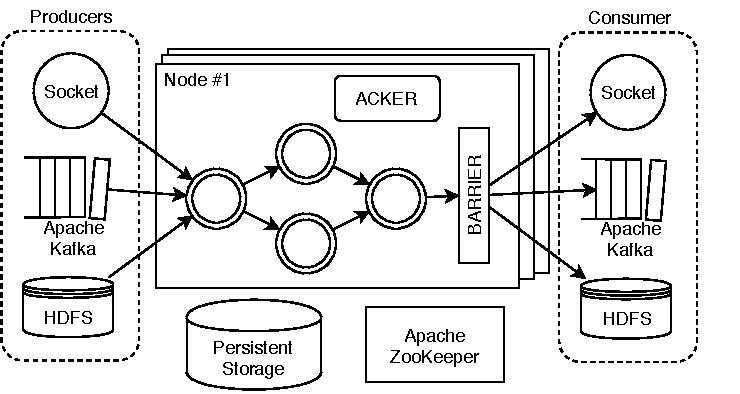
\includegraphics[width=0.70\textwidth]{pics/arch}
  \caption{The overall scheme of the system components}
  \label {system-architecture}
\end{figure}

\subsection{Ordering model}
The meta-information of data item is implemented as a tuple of a {\it global time}, a {\it trace}, {\it child ids} and a {\it tombstone flag}.

\[Meta := (GlobalTime, ChildIds[\:], Trace, IsTombstone)\]

Global time is assigned to data item once the item enters the system. It is a pair of logical time and the identifier of the front. The identifier is used to resolve time collisions within different fronts. It is important to notice that we do not rely on any clock synchronization between nodes. The only implication of the clock skew is the system degradation regarding latency: 1 ms of the fronts clock difference appends 1 ms to minimal latency.

Each map operation can produce multiple items from one.  An ordinal number, child id, is stored in the meta information to differentiate them. {\it ChildIds} is an array of child ids, that corresponds to all visited map operations.

The global time and child ids are enough to uniquely identify data item within a stream if all processing is done in-order. If we compare $(GlobalTime, ChildIds[\:])$ lexicographicaly it has the desired properties that were defined in section~\ref{model-section}. If any grouping repairs happened during processing, multiple items with different payloads but with the same global time and child ids exist in the stream.

To match tombstone item with an invalidated item without payload comparison, there is {\it Trace} value stored in the meta-information that identifies elements path. The unique random 64-bit identifier is assigned to each physical operation. The trace is a xor of all operations' ids visited by item so far. Invalid item and the corresponding tombstone go along the same path, because they have the same payload and the balancing functions are deterministic, so they have the same trace values. Items with the same global times, child ids and traces are guaranteed to have equal payloads.

\label{mininal-time}

\subsection{Minimal time within stream}

To release an item from the barrier we need to ensure that there are no in-flight tombstones for that item, i.e., tombstones which have been already generated, but have not arrived at the barrier yet.

\newtheorem{minimal-time-claim}{Lemma}

\begin{minimal-time-claim}
For any data item $D$ let $\mathcal{G} (D)$ be its global time. 
  If data item $D$ has global time $\mathcal{G} (D) < \mathcal{G} (F)$ for each in-flight element $F$, 
  then all tombstones for that item had already arrived at the barrier.
\end{minimal-time-claim}

\begin{proof}
  Let $D_{tomb}$ be a tombstone for {\it D}. 
  According to the definition of the tombstone item, $\mathcal{G} (D_{tomb}) = \mathcal{G} (D)$, hence $D_{tomb}$ is not in-flight.
  
  New tombstones for $D$ cannot be generated because items with global time greater than $\mathcal{G} (D)$ cannot trigger repair that affects $D$,
  This implies that if the stream does not contain items $D\prime$ such that $\mathcal{G} (D\prime) \le \mathcal{G} (D)$, then all tombstones for $D$ had already arrived at the barrier. 
\end{proof}

Therefore, to output an item from the barrier, we should ensure that there are no items in the stream with the global time less than or equal to the global time of this item.

To track the global time of in-flight items we adopt an idea of {\it acker task} inspired by Apache Storm~\cite{apache:storm}. Acker tracks data items using a checksum hash, called {\it XOR}. When the item is sent or received by an operation, its global time and checksum are sent to the acker. This message is called {\it ack}.
 Acker groups acks by a global time and xors received checksum hashes. 
When an item is sent and later received by the next operation, xoring corresponding {\it XOR}s would yield 0.

Acks are overlapped to nullify {\it XOR} only when an item arrives at the barrier. That is, ack for receive is sent only after both processing and the ack sending for the transformed item are done, as illustrated in Figure~\ref{acker}. This technique guarantees that the {\it XOR} for some global time is equal to zero only if there are no in-flight elements with such global time.

\begin{figure}[ht]
  \centering
  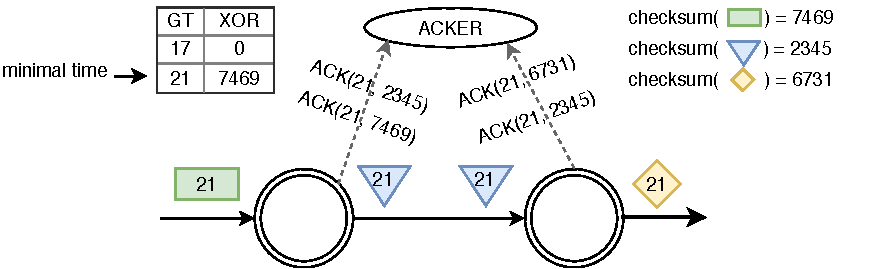
\includegraphics[width=0.8\textwidth]{pics/acker}
  \caption{The example of tracking minimal time using acker}
  \label {acker}
\end{figure}

The minimal time within a stream is the minimal global time with non-zero {\it XOR}. On minimal time changes, acker broadcasts the {\it new minimal time notification}. 
Therefore, the barrier can release elements with global time $\mathcal{G} (D)$ 
once it received notification with time greater than $\mathcal{G} (D)$.

To ensure that no fronts can generate item with the specific timestamp, each front periodically sends to acker a special message called {\it heartbeat} indicating that front will not issue items with a timestamp lower than the reported. The value in the ack table can become zero only after the corresponding heartbeat arrives.
